\documentclass[tikz,border=5pt]{standalone}
\usepackage[utf8]{inputenc}
\usepackage[T1]{fontenc}
\usepackage{lmodern,amsmath,amssymb}
\usepackage[american]{circuitikz}
\usepackage{pgfplots}
\pgfplotsset{compat=1.18}
\usetikzlibrary{circuits.logic.US,positioning,calc,arrows.meta,patterns,shapes.geometric}
\definecolor{Primary}{HTML}{1F77B4}
\begin{document}
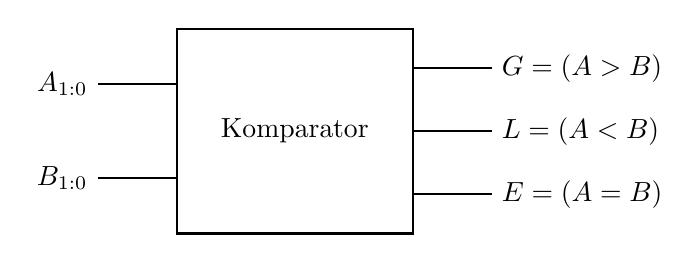
\begin{tikzpicture}[thick]
\draw (0,0) rectangle (3,2.6);\node at (1.5,1.3){Komparator};
\draw (-1,1.9) node[left]{$A_{1:0}$}--(0,1.9);\draw (-1,.7) node[left]{$B_{1:0}$}--(0,.7);
\foreach \y/\t in {2.1/G=(A>B),1.3/L=(A<B),.5/E=(A=B)}{\draw (3,\y)--(4,\y) node[right]{$\t$};}
\end{tikzpicture}
\end{document}
